% 08b_fi_measures_floats.tex -- the floats of the feature-importance measures in 08_feature_importance.tex (2026-10-15):
% lasso selection counts, ridge coefficient mass, the trees' per-refit SHAP rankings and their SHAP interactions.
% Generator: writeup/make_rehaul_fi.py, from results/rehaul_fi/ (experiments/rehaul_fi_compute.py). Labels:
% tab:rh_fi_summary, tab:rh_fi_linear, tab:rh_fi_trees, tab:rh_fi_inter, fig:rh_fi_linear, fig:rh_fi_ranks,
% fig:rh_fi_inter. Prose macros \rhfi...: generated/rehaul_fi_numbers.tex (loaded here too, for a standalone build).
\ifdefined\rhfiNRefits\else% AUTO-GENERATED by writeup/make_rehaul_fi.py -- do not edit; re-run the script.
% \rhfi... macros for writeup/rehaul/08_feature_importance.tex (results/rehaul_fi/).
\providecommand{\rhfiNRefits}{}\renewcommand{\rhfiNRefits}{147}  % refits, one every 10 sessions
\providecommand{\rhfiNOos}{}\renewcommand{\rhfiNOos}{1{,}469}  % scored held-out sessions
\providecommand{\rhfiP}{}\renewcommand{\rhfiP}{628}  % columns, all features
\providecommand{\rhfiNUnits}{}\renewcommand{\rhfiNUnits}{49}  % units: 47 exogenous series + HAR ladder + calendar
\providecommand{\rhfiNExog}{}\renewcommand{\rhfiNExog}{47}  % exogenous series
\providecommand{\rhfiFirst}{}\renewcommand{\rhfiFirst}{25~June~2018}  % first scored session
\providecommand{\rhfiLast}{}\renewcommand{\rhfiLast}{30~April~2024}  % last scored session
\providecommand{\rhfiWindow}{}\renewcommand{\rhfiWindow}{2{,}000}  % sessions in a training window
\providecommand{\rhfiRefitEvery}{}\renewcommand{\rhfiRefitEvery}{10}  % sessions between refits
\providecommand{\rhfiBackbonePf}{}\renewcommand{\rhfiBackbonePf}{0.01}  % backbone penalty factor
\providecommand{\rhfiNBuckets}{}\renewcommand{\rhfiNBuckets}{8}  % exogenous buckets
\providecommand{\rhfiOldBlock}{}\renewcommand{\rhfiOldBlock}{250}  % sessions between the old arm's penalty re-choices
\providecommand{\rhfiNPairs}{}\renewcommand{\rhfiNPairs}{1{,}176}  % series pairs
\providecommand{\rhfiNProbeCols}{}\renewcommand{\rhfiNProbeCols}{631}  % columns of a probe fit
\providecommand{\rhfiTopWPairs}{}\renewcommand{\rhfiTopWPairs}{50}  % pairs in the interaction W
\providecommand{\rhfiProbeLevels}{}\renewcommand{\rhfiProbeLevels}{20}  % values of the few-valued noise column
\providecommand{\rhfiRidgeAlpha}{}\renewcommand{\rhfiRidgeAlpha}{\ensuremath{10^{3}}}
\providecommand{\rhfiLassoAlpha}{}\renewcommand{\rhfiLassoAlpha}{\ensuremath{10^{-2}}}
\providecommand{\rhfiLassoNzMed}{}\renewcommand{\rhfiLassoNzMed}{30}  % median nonzero coefficients per refit
\providecommand{\rhfiLassoNzMin}{}\renewcommand{\rhfiLassoNzMin}{27}
\providecommand{\rhfiLassoNzMax}{}\renewcommand{\rhfiLassoNzMax}{35}
\providecommand{\rhfiLassoExogNzMed}{}\renewcommand{\rhfiLassoExogNzMed}{14}  % ... exogenous columns
\providecommand{\rhfiLassoColsEver}{}\renewcommand{\rhfiLassoColsEver}{60}  % columns nonzero in >= 1 refit
\providecommand{\rhfiLassoColsMajority}{}\renewcommand{\rhfiLassoColsMajority}{29}  % columns nonzero in >= half the refits
\providecommand{\rhfiLassoExogEver}{}\renewcommand{\rhfiLassoExogEver}{27}  % exogenous series with a nonzero column in >= 1 refit
\providecommand{\rhfiLassoExogMajority}{}\renewcommand{\rhfiLassoExogMajority}{11}  % ... in >= half the refits
\providecommand{\rhfiLassoExogAlways}{}\renewcommand{\rhfiLassoExogAlways}{3}  % ... in every refit
\providecommand{\rhfiLassoAlwaysList}{}\renewcommand{\rhfiLassoAlwaysList}{\texttt{sumret}, \texttt{sumabsret\_vwstock}, \texttt{sumautocov}}  % exogenous series selected in every refit
\providecommand{\rhfiLassoProbeSel}{}\renewcommand{\rhfiLassoProbeSel}{1}  % continuous probe selected, of the probe fits
\providecommand{\rhfiLassoProbeSelLevels}{}\renewcommand{\rhfiLassoProbeSelLevels}{0}
\providecommand{\rhfiLassoProbeSelBinary}{}\renewcommand{\rhfiLassoProbeSelBinary}{0}
\providecommand{\rhfiNProbe}{}\renewcommand{\rhfiNProbe}{49}  % probe refits (every third)
\providecommand{\rhfiLassoW}{}\renewcommand{\rhfiLassoW}{0.74}  % Kendall W of the per-refit series ranks by sum |beta|
\providecommand{\rhfiLassoBackboneShare}{}\renewcommand{\rhfiLassoBackboneShare}{88}  % median share of sum |beta| on the backbone, %
\providecommand{\rhfiOldLassoSpearman}{}\renewcommand{\rhfiOldLassoSpearman}{0.70}  % Spearman, selection share: pre-tuned vs re-tuned one-penalty lasso
\providecommand{\rhfiOldLassoNzMed}{}\renewcommand{\rhfiOldLassoNzMed}{23}  % re-tuned lasso: median nonzero per refit
\providecommand{\rhfiOldLassoExogMajority}{}\renewcommand{\rhfiOldLassoExogMajority}{18}
\providecommand{\rhfiRidgeTopOne}{}\renewcommand{\rhfiRidgeTopOne}{Calendar}
\providecommand{\rhfiRidgeTopOneShare}{}\renewcommand{\rhfiRidgeTopOneShare}{31.0}  % % of sum |beta|
\providecommand{\rhfiRidgeTopTwo}{}\renewcommand{\rhfiRidgeTopTwo}{HAR ladder}
\providecommand{\rhfiRidgeTopTwoShare}{}\renewcommand{\rhfiRidgeTopTwoShare}{22.8}  % % of sum |beta|
\providecommand{\rhfiRidgeTopThree}{}\renewcommand{\rhfiRidgeTopThree}{\texttt{sumret}}
\providecommand{\rhfiRidgeTopThreeShare}{}\renewcommand{\rhfiRidgeTopThreeShare}{3.6}  % % of sum |beta|
\providecommand{\rhfiRidgeTopFour}{}\renewcommand{\rhfiRidgeTopFour}{\texttt{sumabsret\_vwstock}}
\providecommand{\rhfiRidgeTopFourShare}{}\renewcommand{\rhfiRidgeTopFourShare}{2.2}  % % of sum |beta|
\providecommand{\rhfiRidgeSdTopOne}{}\renewcommand{\rhfiRidgeSdTopOne}{HAR ladder}
\providecommand{\rhfiRidgeSdTopOneShare}{}\renewcommand{\rhfiRidgeSdTopOneShare}{30.6}  % % of sum |beta| sd
\providecommand{\rhfiRidgeSdTopTwo}{}\renewcommand{\rhfiRidgeSdTopTwo}{Calendar}
\providecommand{\rhfiRidgeSdTopTwoShare}{}\renewcommand{\rhfiRidgeSdTopTwoShare}{9.3}  % % of sum |beta| sd
\providecommand{\rhfiRidgeSdTopThree}{}\renewcommand{\rhfiRidgeSdTopThree}{\texttt{sumret}}
\providecommand{\rhfiRidgeSdTopThreeShare}{}\renewcommand{\rhfiRidgeSdTopThreeShare}{4.5}  % % of sum |beta| sd
\providecommand{\rhfiRidgeTopExog}{}\renewcommand{\rhfiRidgeTopExog}{\texttt{sumret}}
\providecommand{\rhfiRidgeTopExogShare}{}\renewcommand{\rhfiRidgeTopExogShare}{3.6}
\providecommand{\rhfiRidgeBackboneShare}{}\renewcommand{\rhfiRidgeBackboneShare}{54}  % median share of sum |beta| on the backbone, %
\providecommand{\rhfiRidgeW}{}\renewcommand{\rhfiRidgeW}{0.85}
\providecommand{\rhfiRidgeAllSelected}{}\renewcommand{\rhfiRidgeAllSelected}{49}  % units with N_A = K under the ridge
\providecommand{\rhfiLassoProbeRate}{}\renewcommand{\rhfiLassoProbeRate}{2.0}  % continuous probe's selection rate, %
\providecommand{\rhfiLassoColsAboveProbe}{}\renewcommand{\rhfiLassoColsAboveProbe}{54}  % columns selected more often than the continuous probe
\providecommand{\rhfiLassoSeriesAboveProbe}{}\renewcommand{\rhfiLassoSeriesAboveProbe}{23}  % exogenous series with such a column
\providecommand{\rhfiLassoTopCol}{}\renewcommand{\rhfiLassoTopCol}{\texttt{is\_month\_end}}
\providecommand{\rhfiRidgeSpearmanSd}{}\renewcommand{\rhfiRidgeSpearmanSd}{0.85}  % Spearman, series sum|beta| vs sum|beta| sd
\providecommand{\rhfiRidgeProbeBeat}{}\renewcommand{\rhfiRidgeProbeBeat}{107}  % columns with |beta| above the continuous probe's in most probe fits
\providecommand{\rhfiRidgeProbeBeatSeries}{}\renewcommand{\rhfiRidgeProbeBeatSeries}{38}
\providecommand{\rhfiScaleValueN}{}\renewcommand{\rhfiScaleValueN}{282}
\providecommand{\rhfiScaleValueSd}{}\renewcommand{\rhfiScaleValueSd}{0.84}  % median window sd, value ladders
\providecommand{\rhfiScaleValueSdLo}{}\renewcommand{\rhfiScaleValueSdLo}{0.03}
\providecommand{\rhfiScaleValueSdHi}{}\renewcommand{\rhfiScaleValueSdHi}{1.76}
\providecommand{\rhfiScaleValueIqr}{}\renewcommand{\rhfiScaleValueIqr}{0.94}  % median window IQR, value ladders
\providecommand{\rhfiScaleFlagN}{}\renewcommand{\rhfiScaleFlagN}{324}
\providecommand{\rhfiScaleFlagSd}{}\renewcommand{\rhfiScaleFlagSd}{0.022}  % median window sd, availability / activity ladders
\providecommand{\rhfiScaleFlagSdHi}{}\renewcommand{\rhfiScaleFlagSdHi}{0.17}
\providecommand{\rhfiScaleCalSd}{}\renewcommand{\rhfiScaleCalSd}{0.39}  % median window sd, calendar
\providecommand{\rhfiScaleHarSd}{}\renewcommand{\rhfiScaleHarSd}{1.07}  % median window sd, HAR ladder
\providecommand{\rhfiLgbmW}{}\renewcommand{\rhfiLgbmW}{0.57}  % lgbm: Kendall W, per-refit series ranks
\providecommand{\rhfiLgbmWCols}{}\renewcommand{\rhfiLgbmWCols}{0.91}  % lgbm: Kendall W, column ranks
\providecommand{\rhfiLgbmTopOne}{}\renewcommand{\rhfiLgbmTopOne}{HAR ladder}
\providecommand{\rhfiLgbmTopOneRank}{}\renewcommand{\rhfiLgbmTopOneRank}{1.0}  % mean rank
\providecommand{\rhfiLgbmTopTwo}{}\renewcommand{\rhfiLgbmTopTwo}{\texttt{sumret}}
\providecommand{\rhfiLgbmTopTwoRank}{}\renewcommand{\rhfiLgbmTopTwoRank}{2.9}  % mean rank
\providecommand{\rhfiLgbmTopThree}{}\renewcommand{\rhfiLgbmTopThree}{\texttt{sumabsret}}
\providecommand{\rhfiLgbmTopThreeRank}{}\renewcommand{\rhfiLgbmTopThreeRank}{4.8}  % mean rank
\providecommand{\rhfiLgbmSpBorda}{}\renewcommand{\rhfiLgbmSpBorda}{0.90}  % Spearman, mean rank vs top-10 Borda
\providecommand{\rhfiLgbmSpGlobal}{}\renewcommand{\rhfiLgbmSpGlobal}{0.96}  % Spearman, mean rank vs global mean |phi|
\providecommand{\rhfiLgbmSpLocal}{}\renewcommand{\rhfiLgbmSpLocal}{1.000}  % Spearman, mean ranks local refit vs stored
\providecommand{\rhfiLgbmProbeRank}{}\renewcommand{\rhfiLgbmProbeRank}{83}  % median rank of the continuous probe, 631 columns
\providecommand{\rhfiLgbmProbeCols}{}\renewcommand{\rhfiLgbmProbeCols}{60}  % columns above the continuous probe in most probe fits
\providecommand{\rhfiLgbmProbeSeries}{}\renewcommand{\rhfiLgbmProbeSeries}{27}  % exogenous series with such a column
\providecommand{\rhfiLgbmTopCol}{}\renewcommand{\rhfiLgbmTopCol}{\texttt{har\_ma\_1}}  % column with the lowest mean rank
\providecommand{\rhfiLgbmTopColRank}{}\renewcommand{\rhfiLgbmTopColRank}{1.3}
\providecommand{\rhfiLgbmTopColTwo}{}\renewcommand{\rhfiLgbmTopColTwo}{\texttt{har\_ma\_5}}
\providecommand{\rhfiLgbmTopColTwoRank}{}\renewcommand{\rhfiLgbmTopColTwoRank}{1.8}
\providecommand{\rhfiLgbmPredGap}{}\renewcommand{\rhfiLgbmPredGap}{0}  % max |local refit - stored refit| forecast
\providecommand{\rhfiLgbmInterW}{}\renewcommand{\rhfiLgbmInterW}{0.45}  % Kendall W of per-refit pair ranks, top-50 pairs
\providecommand{\rhfiLgbmInterRatio}{}\renewcommand{\rhfiLgbmInterRatio}{90}  % sum of series-pair interactions / sum main, %
\providecommand{\rhfiLgbmInterSpGlobal}{}\renewcommand{\rhfiLgbmInterSpGlobal}{0.99}
\providecommand{\rhfiLgbmInterFloor}{}\renewcommand{\rhfiLgbmInterFloor}{0.49}  % probe floor x 1e3
\providecommand{\rhfiLgbmInterAboveFloor}{}\renewcommand{\rhfiLgbmInterAboveFloor}{116}  % series pairs above the probe floor
\providecommand{\rhfiLgbmInterTopA}{}\renewcommand{\rhfiLgbmInterTopA}{HAR ladder}
\providecommand{\rhfiLgbmInterTopB}{}\renewcommand{\rhfiLgbmInterTopB}{\texttt{sumabsret}}
\providecommand{\rhfiLgbmInterTopVal}{}\renewcommand{\rhfiLgbmInterTopVal}{12.6}  % x 1e3
\providecommand{\rhfiLgbmHTop}{}\renewcommand{\rhfiLgbmHTop}{0.33}  % H^2 of the top series pair (pooled), %
\providecommand{\rhfiLgbmHMin}{}\renewcommand{\rhfiLgbmHMin}{0.02}  % min H^2 over the top-10 series pairs, %
\providecommand{\rhfiLgbmHMax}{}\renewcommand{\rhfiLgbmHMax}{0.33}  % max H^2 over the top-10 series pairs, %
\providecommand{\rhfiLgbmHMinTop}{}\renewcommand{\rhfiLgbmHMinTop}{0.19}  % top pair: interaction PD var / smaller main PD var
\providecommand{\rhfiLgbmHMinLo}{}\renewcommand{\rhfiLgbmHMinLo}{0.05}  % ... min over the top-10 series pairs
\providecommand{\rhfiLgbmHMinHi}{}\renewcommand{\rhfiLgbmHMinHi}{0.54}  % ... max
\providecommand{\rhfiLgbmHColTop}{}\renewcommand{\rhfiLgbmHColTop}{0.36}  % H^2 of the top column pair, %
\providecommand{\rhfiLgbmHMinColTop}{}\renewcommand{\rhfiLgbmHMinColTop}{0.02}  % ... min-normalised
\providecommand{\rhfiLgbmMainTopVal}{}\renewcommand{\rhfiLgbmMainTopVal}{195}  % largest global mean |phi_A| x 1e3
\providecommand{\rhfiLgbmWithinTop}{}\renewcommand{\rhfiLgbmWithinTop}{HAR ladder}
\providecommand{\rhfiLgbmWithinTopVal}{}\renewcommand{\rhfiLgbmWithinTopVal}{18.7}
\providecommand{\rhfiXgbW}{}\renewcommand{\rhfiXgbW}{0.60}  % xgb: Kendall W, per-refit series ranks
\providecommand{\rhfiXgbWCols}{}\renewcommand{\rhfiXgbWCols}{0.90}  % xgb: Kendall W, column ranks
\providecommand{\rhfiXgbTopOne}{}\renewcommand{\rhfiXgbTopOne}{HAR ladder}
\providecommand{\rhfiXgbTopOneRank}{}\renewcommand{\rhfiXgbTopOneRank}{1.0}  % mean rank
\providecommand{\rhfiXgbTopTwo}{}\renewcommand{\rhfiXgbTopTwo}{\texttt{sumret}}
\providecommand{\rhfiXgbTopTwoRank}{}\renewcommand{\rhfiXgbTopTwoRank}{3.0}  % mean rank
\providecommand{\rhfiXgbTopThree}{}\renewcommand{\rhfiXgbTopThree}{\texttt{sumabsret}}
\providecommand{\rhfiXgbTopThreeRank}{}\renewcommand{\rhfiXgbTopThreeRank}{3.9}  % mean rank
\providecommand{\rhfiXgbSpBorda}{}\renewcommand{\rhfiXgbSpBorda}{0.87}  % Spearman, mean rank vs top-10 Borda
\providecommand{\rhfiXgbSpGlobal}{}\renewcommand{\rhfiXgbSpGlobal}{0.97}  % Spearman, mean rank vs global mean |phi|
\providecommand{\rhfiXgbSpLocal}{}\renewcommand{\rhfiXgbSpLocal}{0.993}  % Spearman, mean ranks local refit vs stored
\providecommand{\rhfiXgbProbeRank}{}\renewcommand{\rhfiXgbProbeRank}{110}  % median rank of the continuous probe, 631 columns
\providecommand{\rhfiXgbProbeCols}{}\renewcommand{\rhfiXgbProbeCols}{78}  % columns above the continuous probe in most probe fits
\providecommand{\rhfiXgbProbeSeries}{}\renewcommand{\rhfiXgbProbeSeries}{35}  % exogenous series with such a column
\providecommand{\rhfiXgbTopCol}{}\renewcommand{\rhfiXgbTopCol}{\texttt{har\_ma\_1}}  % column with the lowest mean rank
\providecommand{\rhfiXgbTopColRank}{}\renewcommand{\rhfiXgbTopColRank}{1.3}
\providecommand{\rhfiXgbTopColTwo}{}\renewcommand{\rhfiXgbTopColTwo}{\texttt{har\_ma\_5}}
\providecommand{\rhfiXgbTopColTwoRank}{}\renewcommand{\rhfiXgbTopColTwoRank}{1.8}
\providecommand{\rhfiXgbPredGap}{}\renewcommand{\rhfiXgbPredGap}{0.17}  % max |local refit - stored refit| forecast
\providecommand{\rhfiXgbInterW}{}\renewcommand{\rhfiXgbInterW}{0.47}  % Kendall W of per-refit pair ranks, top-50 pairs
\providecommand{\rhfiXgbInterRatio}{}\renewcommand{\rhfiXgbInterRatio}{74}  % sum of series-pair interactions / sum main, %
\providecommand{\rhfiXgbInterSpGlobal}{}\renewcommand{\rhfiXgbInterSpGlobal}{0.99}
\providecommand{\rhfiXgbInterFloor}{}\renewcommand{\rhfiXgbInterFloor}{0.41}  % probe floor x 1e3
\providecommand{\rhfiXgbInterAboveFloor}{}\renewcommand{\rhfiXgbInterAboveFloor}{115}  % series pairs above the probe floor
\providecommand{\rhfiXgbInterTopA}{}\renewcommand{\rhfiXgbInterTopA}{HAR ladder}
\providecommand{\rhfiXgbInterTopB}{}\renewcommand{\rhfiXgbInterTopB}{\texttt{sumabsret}}
\providecommand{\rhfiXgbInterTopVal}{}\renewcommand{\rhfiXgbInterTopVal}{15.2}  % x 1e3
\providecommand{\rhfiXgbHTop}{}\renewcommand{\rhfiXgbHTop}{0.37}  % H^2 of the top series pair (pooled), %
\providecommand{\rhfiXgbHMin}{}\renewcommand{\rhfiXgbHMin}{0.02}  % min H^2 over the top-10 series pairs, %
\providecommand{\rhfiXgbHMax}{}\renewcommand{\rhfiXgbHMax}{0.68}  % max H^2 over the top-10 series pairs, %
\providecommand{\rhfiXgbHMinTop}{}\renewcommand{\rhfiXgbHMinTop}{0.39}  % top pair: interaction PD var / smaller main PD var
\providecommand{\rhfiXgbHMinLo}{}\renewcommand{\rhfiXgbHMinLo}{0.08}  % ... min over the top-10 series pairs
\providecommand{\rhfiXgbHMinHi}{}\renewcommand{\rhfiXgbHMinHi}{0.80}  % ... max
\providecommand{\rhfiXgbHColTop}{}\renewcommand{\rhfiXgbHColTop}{0.39}  % H^2 of the top column pair, %
\providecommand{\rhfiXgbHMinColTop}{}\renewcommand{\rhfiXgbHMinColTop}{0.02}  % ... min-normalised
\providecommand{\rhfiXgbMainTopVal}{}\renewcommand{\rhfiXgbMainTopVal}{192}  % largest global mean |phi_A| x 1e3
\providecommand{\rhfiXgbWithinTop}{}\renewcommand{\rhfiXgbWithinTop}{HAR ladder}
\providecommand{\rhfiXgbWithinTopVal}{}\renewcommand{\rhfiXgbWithinTopVal}{19.1}
\providecommand{\rhfiRfW}{}\renewcommand{\rhfiRfW}{0.62}  % rf: Kendall W, per-refit series ranks
\providecommand{\rhfiRfWCols}{}\renewcommand{\rhfiRfWCols}{0.93}  % rf: Kendall W, column ranks
\providecommand{\rhfiRfTopOne}{}\renewcommand{\rhfiRfTopOne}{HAR ladder}
\providecommand{\rhfiRfTopOneRank}{}\renewcommand{\rhfiRfTopOneRank}{1.0}  % mean rank
\providecommand{\rhfiRfTopTwo}{}\renewcommand{\rhfiRfTopTwo}{\texttt{sumabsret}}
\providecommand{\rhfiRfTopTwoRank}{}\renewcommand{\rhfiRfTopTwoRank}{2.6}  % mean rank
\providecommand{\rhfiRfTopThree}{}\renewcommand{\rhfiRfTopThree}{\texttt{sumret}}
\providecommand{\rhfiRfTopThreeRank}{}\renewcommand{\rhfiRfTopThreeRank}{4.0}  % mean rank
\providecommand{\rhfiRfSpBorda}{}\renewcommand{\rhfiRfSpBorda}{0.92}  % Spearman, mean rank vs top-10 Borda
\providecommand{\rhfiRfSpGlobal}{}\renewcommand{\rhfiRfSpGlobal}{0.98}  % Spearman, mean rank vs global mean |phi|
\providecommand{\rhfiRfSpLocal}{}\renewcommand{\rhfiRfSpLocal}{0.996}  % Spearman, mean ranks local refit vs stored
\providecommand{\rhfiRfProbeRank}{}\renewcommand{\rhfiRfProbeRank}{97}  % median rank of the continuous probe, 631 columns
\providecommand{\rhfiRfProbeCols}{}\renewcommand{\rhfiRfProbeCols}{71}  % columns above the continuous probe in most probe fits
\providecommand{\rhfiRfProbeSeries}{}\renewcommand{\rhfiRfProbeSeries}{29}  % exogenous series with such a column
\providecommand{\rhfiRfTopCol}{}\renewcommand{\rhfiRfTopCol}{\texttt{har\_ma\_1}}  % column with the lowest mean rank
\providecommand{\rhfiRfTopColRank}{}\renewcommand{\rhfiRfTopColRank}{1.3}
\providecommand{\rhfiRfTopColTwo}{}\renewcommand{\rhfiRfTopColTwo}{\texttt{har\_ma\_5}}
\providecommand{\rhfiRfTopColTwoRank}{}\renewcommand{\rhfiRfTopColTwoRank}{1.7}
\providecommand{\rhfiRfPredGap}{}\renewcommand{\rhfiRfPredGap}{0.11}  % max |local refit - stored refit| forecast
\providecommand{\rhfiRfInterW}{}\renewcommand{\rhfiRfInterW}{0.57}  % Kendall W of per-refit pair ranks, top-50 pairs
\providecommand{\rhfiRfInterRatio}{}\renewcommand{\rhfiRfInterRatio}{72}  % sum of series-pair interactions / sum main, %
\providecommand{\rhfiRfInterSpGlobal}{}\renewcommand{\rhfiRfInterSpGlobal}{1.00}
\providecommand{\rhfiRfInterFloor}{}\renewcommand{\rhfiRfInterFloor}{0.50}  % probe floor x 1e3
\providecommand{\rhfiRfInterAboveFloor}{}\renewcommand{\rhfiRfInterAboveFloor}{52}  % series pairs above the probe floor
\providecommand{\rhfiRfInterTopA}{}\renewcommand{\rhfiRfInterTopA}{HAR ladder}
\providecommand{\rhfiRfInterTopB}{}\renewcommand{\rhfiRfInterTopB}{\texttt{sumabsret}}
\providecommand{\rhfiRfInterTopVal}{}\renewcommand{\rhfiRfInterTopVal}{23.8}  % x 1e3
\providecommand{\rhfiRfHTop}{}\renewcommand{\rhfiRfHTop}{0.85}  % H^2 of the top series pair (pooled), %
\providecommand{\rhfiRfHMin}{}\renewcommand{\rhfiRfHMin}{0.02}  % min H^2 over the top-10 series pairs, %
\providecommand{\rhfiRfHMax}{}\renewcommand{\rhfiRfHMax}{0.85}  % max H^2 over the top-10 series pairs, %
\providecommand{\rhfiRfHMinTop}{}\renewcommand{\rhfiRfHMinTop}{1.50}  % top pair: interaction PD var / smaller main PD var
\providecommand{\rhfiRfHMinLo}{}\renewcommand{\rhfiRfHMinLo}{0.17}  % ... min over the top-10 series pairs
\providecommand{\rhfiRfHMinHi}{}\renewcommand{\rhfiRfHMinHi}{5.46}  % ... max
\providecommand{\rhfiRfHColTop}{}\renewcommand{\rhfiRfHColTop}{1.16}  % H^2 of the top column pair, %
\providecommand{\rhfiRfHMinColTop}{}\renewcommand{\rhfiRfHMinColTop}{0.06}  % ... min-normalised
\providecommand{\rhfiRfMainTopVal}{}\renewcommand{\rhfiRfMainTopVal}{224}  % largest global mean |phi_A| x 1e3
\providecommand{\rhfiRfWithinTop}{}\renewcommand{\rhfiRfWithinTop}{HAR ladder}
\providecommand{\rhfiRfWithinTopVal}{}\renewcommand{\rhfiRfWithinTopVal}{34.3}
\providecommand{\rhfiSpTreesMin}{}\renewcommand{\rhfiSpTreesMin}{0.83}  % Spearman of mean ranks, trees
\providecommand{\rhfiSpTreesMax}{}\renewcommand{\rhfiSpTreesMax}{0.96}
\providecommand{\rhfiSpTreeLinMin}{}\renewcommand{\rhfiSpTreeLinMin}{0.17}  % Spearman of mean ranks, tree vs linear
\providecommand{\rhfiSpTreeLinMax}{}\renewcommand{\rhfiSpTreeLinMax}{0.55}
\providecommand{\rhfiSpLassoRidge}{}\renewcommand{\rhfiSpLassoRidge}{0.47}
\providecommand{\rhfiHRefits}{}\renewcommand{\rhfiHRefits}{15}  % refits for H
\providecommand{\rhfiHRows}{}\renewcommand{\rhfiHRows}{100}  % evaluation points per refit
\providecommand{\rhfiHTopSeries}{}\renewcommand{\rhfiHTopSeries}{10}
\providecommand{\rhfiFitSecRf}{}\renewcommand{\rhfiFitSecRf}{212}  % mean seconds per forest refit (11 processes sharing the CPU)
\providecommand{\rhfiShapSecRf}{}\renewcommand{\rhfiShapSecRf}{182}  % mean seconds per forest refit, SHAP + interactions
\providecommand{\rhfiShapSecLgbm}{}\renewcommand{\rhfiShapSecLgbm}{0.9}  % ... LightGBM
\providecommand{\rhfiShapSecXgb}{}\renewcommand{\rhfiShapSecXgb}{0.4}  % ... XGBoost
\providecommand{\rhfiWallTreesMin}{}\renewcommand{\rhfiWallTreesMin}{133}  % wall minutes, tree stage on 11 processes
\providecommand{\rhfiWallHMin}{}\renewcommand{\rhfiWallHMin}{7}  % wall minutes, H stage
\providecommand{\rhfiWallLinMin}{}\renewcommand{\rhfiWallLinMin}{7}  % wall minutes, linear stage
\providecommand{\rhfiWorkers}{}\renewcommand{\rhfiWorkers}{11}
\fi

% One row per model: aggregate measure, leading units, Kendall's W, units above the noise bar
% AUTO-GENERATED by writeup/make_rehaul_fi.py -- do not edit; re-run the script.

\begin{table}[tbp]
\centering
\small
\setlength{\tabcolsep}{4pt}
\begin{threeparttable}
\caption{Feature importance by the coefficient and SHAP measures: the leading units per model, all features.}
\label{tab:rh_fi_summary}
\begin{tabular}{@{}llp{8.4cm}rr@{}}
\toprule
Model & Measure & Leading units & $W$ & Above noise \\
\midrule
Lasso & $N_A$ & Calendar 147; HAR ladder 147; \texttt{sumret} 147 & 0.74 & 23 \\
Ridge & $S_A$ (\%) & Calendar 31.0; HAR ladder 22.8; \texttt{sumret} 3.6 & 0.85 & 38 \\
LightGBM & $\bar r_A$ & HAR ladder 1.0; \texttt{sumret} 2.9; \texttt{sumabsret} 4.8 & 0.57 & 27 \\
XGBoost & $\bar r_A$ & HAR ladder 1.0; \texttt{sumret} 3.0; \texttt{sumabsret} 3.9 & 0.60 & 35 \\
Random forest & $\bar r_A$ & HAR ladder 1.0; \texttt{sumabsret} 2.6; \texttt{sumret} 4.0 & 0.62 & 29 \\
\bottomrule
\end{tabular}
\begin{tablenotes}[flushleft]
\footnotesize
\item \textit{Notes:} Per-bar 16:00 models of record, all features ($p = 628$ columns in 49 units: 47 exogenous series, the HAR ladder and the calendar block), 147 refits, one every 10 sessions. Lasso and ridge: pre-tuned penalties $\alpha = {10^{-2}}$ and ${10^{3}}$, backbone penalised at 1/100. $N_A$: refits in which a column of unit $A$ has $\beta_j \ne 0$; $S_A$: share of $\sum_k \sum_{j} |\beta^{(k)}_j|$ on $A$; $\bar r_A$: mean over refits of $A$'s rank by mean $|\phi_{t,A}|$ on the refit's held-out rows (1 = largest). $W$: Kendall's coefficient of concordance of the per-refit rankings (by $\sum_{j \in A} |\beta_j|$ for the linear models). Noise bar, exogenous series clearing it: lasso, a column selected in a larger share of the refits than the continuous probe in its 49 probe fits (1); ridge, a column with $|\beta_j|$ above the continuous probe's in at least half of the probe fits; trees, a column with mean $|\phi_j|$ above the continuous probe's in at least half of the probe fits.
\end{tablenotes}
\end{threeparttable}
\end{table}


% Lasso N_A and ridge S_A per unit
% AUTO-GENERATED by writeup/make_rehaul_fi.py -- do not edit; re-run the script.

\begin{table}[tbp]
\centering
\small
\setlength{\tabcolsep}{4pt}
\begin{threeparttable}
\caption{Lasso and ridge: how often each unit is selected and its share of the coefficient mass, 147 refits.}
\label{tab:rh_fi_linear}
\begin{tabular}{@{}llrrrrrrr@{}}
\toprule
 & & & \multicolumn{3}{c}{Lasso} & \multicolumn{3}{c}{Ridge} \\
\cmidrule(lr){4-6}\cmidrule(l){7-9}
Unit & Bucket & Cols & $N_A$ & Active & $\sum|\beta|$ (\%) & $\sum|\beta|$ (\%) & $\sum|\beta|\,\mathrm{sd}$ (\%) & Mean rank \\
\midrule
Calendar & BB & 16 & 147 & 10.0 & 53.2 & 31.0 & 9.3 & 1.0 \\
HAR ladder & BB & 6 & 147 & 5.9 & 34.6 & 22.8 & 30.6 & 2.0 \\
\texttt{sumret} & Mom & 12 & 147 & 3.0 & 5.4 & 3.6 & 4.5 & 3.0 \\
\texttt{sumabsret\_vwstock} & VW & 12 & 147 & 1.0 & 2.6 & 2.2 & 3.7 & 4.6 \\
\texttt{sumautocov} & Mom & 12 & 147 & 1.3 & 1.2 & 2.1 & 2.2 & 5.0 \\
\texttt{sumpret2\_ewstock} & EW & 12 & 126 & 1.2 & 0.6 & 1.1 & 1.9 & 17.8 \\
\texttt{effspread\_vwstock} & Liq & 12 & 119 & 0.8 & 0.2 & 1.3 & 2.5 & 13.1 \\
\texttt{sellturnover\_vwstock} & Liq & 12 & 109 & 0.7 & 1.0 & 1.2 & 1.4 & 16.5 \\
\texttt{sumret4} & Mom & 12 & 107 & 0.8 & 0.2 & 1.2 & 2.2 & 15.8 \\
\texttt{sumret4\_vwstock} & VW & 12 & 106 & 0.7 & 0.1 & 0.7 & 1.2 & 34.2 \\
\texttt{sumpret2\_vwstock} & VW & 12 & 105 & 0.8 & 0.2 & 1.0 & 1.7 & 21.2 \\
\texttt{ofi\_ewstock} & Liq & 12 & 83 & 0.8 & 0.1 & 1.5 & 1.5 & 10.4 \\
\texttt{vix} & IV & 12 & 83 & 0.6 & 0.1 & 1.7 & 2.2 & 8.1 \\
\texttt{sumret4\_ewstock} & EW & 12 & 65 & 0.5 & 0.1 & 0.7 & 1.1 & 33.6 \\
\texttt{effspread\_ewstock} & Liq & 12 & 56 & 0.5 & 0.0 & 1.0 & 1.6 & 23.6 \\
\texttt{numobs} & Liq & 18 & 45 & 0.3 & 0.0 & 0.4 & 0.4 & 44.7 \\
\texttt{fomc\_day} & FOMC & 18 & 42 & 0.3 & 0.0 & 0.4 & 0.6 & 44.4 \\
\texttt{spread\_vwstock} & Liq & 12 & 35 & 0.2 & 0.1 & 0.8 & 0.7 & 29.7 \\
\texttt{sumbipow\_ewstock} & EW & 12 & 26 & 0.2 & 0.1 & 0.6 & 1.1 & 37.2 \\
\texttt{sumbipow} & Mom & 12 & 25 & 0.2 & 0.0 & 0.5 & 1.0 & 41.2 \\
\bottomrule
\end{tabular}
\begin{tablenotes}[flushleft]
\footnotesize
\item \textit{Notes:} Units ordered by the lasso's $N_A$ (ties by its $\sum|\beta|$); the first 20 of 49 shown, 20 units are never selected. Cols: columns of the unit. Lasso: $N_A$ = refits (of 147) with a nonzero coefficient on the unit; active = mean number of its nonzero columns; $\sum|\beta|$ = its share of $\sum_k\sum_j|\beta^{(k)}_j|$. Ridge: the same share; $\sum|\beta|\,\mathrm{sd}$ = the share with each $|\beta_j|$ scaled by the column's standard deviation on the refit's 2,000-session window; mean rank = mean over refits of the unit's rank by $\sum_{j\in A}|\beta^{(k)}_j|$. Value ladders are robust-scaled (median window standard deviation 0.84), but the 324 availability and activity ladders are not (0.022), nor the calendar dummies (0.39). Backbone (BB) columns carry 1/100 of the penalty. Buckets: Mom return moments, Liq liquidity, EW / VW equal- / value-weighted market, Sent sentiment, IV implied volatility, VD volatility demand.
\end{tablenotes}
\end{threeparttable}
\end{table}


% The linear coefficients over time (lasso on/off and magnitude; ridge shares)
% 2026-10-15 (user): parked -- non-standard figure; focus on legible tables
% % AUTO-GENERATED by writeup/make_rehaul_fi.py -- do not edit; re-run the script.
\begin{figure}[tbp]
\centering
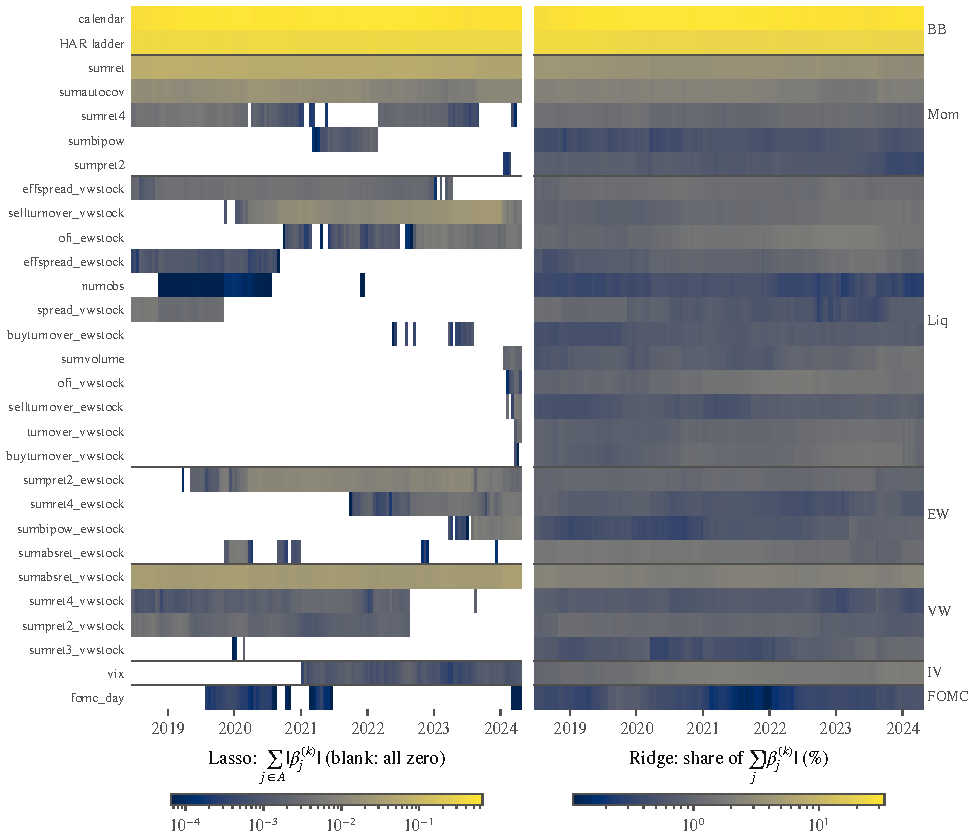
\includegraphics[width=\linewidth]{figures/rehaul_fi_linear_time.pdf}
\caption{The linear coefficients over time, by unit, at the 147 refits (every 10 sessions, 25 June 2018 to 30 April 2024). Left: the pre-tuned lasso's $\sum_{j\in A}|\beta^{(k)}_j|$, log colour scale, blank where every coefficient of the unit is zero (the on/off pattern). Right: the pre-tuned ridge's share of the refit's $\sum_j|\beta^{(k)}_j|$ on the unit, \%. Rows: the 29 units the lasso selects at least once, grouped by bucket (backbone first) and ordered by $N_A$; the other 20 are never selected. Coefficients are per unit of the robust-scaled input (see Table~\ref{tab:rh_fi_linear}).}
\label{fig:rh_fi_linear}
\end{figure}


% Trees: per-refit SHAP ranks aggregated (mean rank, top-5 share, truncated Borda, Kendall's W)
% AUTO-GENERATED by writeup/make_rehaul_fi.py -- do not edit; re-run the script.

\begin{table}[tbp]
\centering
\small
\setlength{\tabcolsep}{3.5pt}
\begin{threeparttable}
\caption{Trees: the per-refit SHAP rankings of the units, aggregated over 147 refits.}
\label{tab:rh_fi_trees}
\begin{tabular}{@{}llrrrrrrrrr@{}}
\toprule
 & & \multicolumn{3}{c}{LightGBM} & \multicolumn{3}{c}{XGBoost} & \multicolumn{3}{c}{Random forest} \\
\cmidrule(lr){3-5}\cmidrule(lr){6-8}\cmidrule(l){9-11}
Unit & Bucket & $\bar r$ & Top 5 & Borda & $\bar r$ & Top 5 & Borda & $\bar r$ & Top 5 & Borda \\
\midrule
HAR ladder & BB & 1.0 & 100 & 1 & 1.0 & 100 & 1 & 1.0 & 100 & 1 \\
\texttt{sumret} & Mom & 2.9 & 97 & 2 & 3.0 & 97 & 2 & 4.0 & 82 & 3 \\
\texttt{sumabsret} & Mom & 4.8 & 71 & 4 & 3.9 & 87 & 3 & 2.6 & 97 & 2 \\
\texttt{sumvolume} & Liq & 4.9 & 71 & 3 & 4.6 & 75 & 4 & 5.1 & 69 & 4 \\
\texttt{sumabsret\_ewstock} & EW & 6.7 & 39 & 5 & 6.7 & 38 & 5 & 5.7 & 46 & 5 \\
\texttt{sumabsret\_vwstock} & VW & 10.0 & 15 & 7 & 8.6 & 13 & 7 & 6.1 & 46 & 6 \\
Calendar & BB & 7.9 & 37 & 6 & 8.1 & 31 & 6 & 15.1 & 7 & 9 \\
\texttt{stocktwits\_sentiment} & Sent & 11.9 & 16 & 8 & 11.6 & 17 & 8 & 11.3 & 19 & 7 \\
\texttt{sumautocov} & Mom & 11.9 & 3 & 10 & 11.6 & 5 & 11 & 16.1 & 2 & 13 \\
\texttt{ofi\_ewstock} & Liq & 14.6 & 14 & 9 & 14.8 & 11 & 9 & 12.9 & 9 & 8 \\
\texttt{sumret3} & Mom & 17.9 & 3 & 13 & 16.5 & 1 & 13 & 15.4 & 2 & 12 \\
\texttt{stocktwits\_sentcount} & Sent & 17.1 & 7 & 11 & 16.2 & 4 & 12 & 17.6 & 3 & 11 \\
\texttt{sellturnover\_vwstock} & Liq & 20.0 & 7 & 12 & 16.4 & 8 & 10 & 18.3 & 7 & 10 \\
\texttt{ofi\_vwstock} & Liq & 25.8 & 1 & 24 & 26.0 & 2 & 19 & 18.4 & 1 & 15 \\
\texttt{stocktwits\_attention} & Sent & 22.7 & 1 & 20 & 24.4 & 1 & 18 & 23.7 & 0 & 19 \\
\addlinespace[3pt]
Kendall's $W$ & & \multicolumn{3}{c}{0.57} & \multicolumn{3}{c}{0.60} & \multicolumn{3}{c}{0.62} \\
Exog.\ series above the probe & & \multicolumn{3}{c}{27} & \multicolumn{3}{c}{35} & \multicolumn{3}{c}{29} \\
\bottomrule
\end{tabular}
\begin{tablenotes}[flushleft]
\footnotesize
\item \textit{Notes:} Per refit $k$, unit $A$'s importance is $I_{k,A} = |T_k|^{-1}\sum_{t\in T_k}|\phi_{t,A}|$, $\phi_{t,A} = \sum_{j\in A}\phi_{t,j}$ (path-dependent TreeSHAP of the refit's model on its held-out rows); $r_{k,A}$ is its rank among the 49 units (1 = largest, ties averaged). $\bar r$: mean of $r_{k,A}$ over the 147 refits; top 5: share of refits with $r_{k,A} \le 5$, \%; Borda: rank of $\sum_k \max(0, 11 - r_{k,A})$ (a full Borda count is affine in $\bar r$). Units: the 15 with the lowest $\bar r$ averaged over the three models. Kendall's $W$ of the per-refit rankings ($W = 1$: identical rankings at every refit). Probe: an exogenous series counts if one of its columns has mean $|\phi_j|$ above the continuous noise column's in at least half of the 49 probe fits (every third refit). SHAP values are the de-dup study's stored values of the cluster refits (LightGBM lgbm\_opt\_00, XGBoost xgb\_opt\_00, random forest trial 255, window-masked).
\end{tablenotes}
\end{threeparttable}
\end{table}


% Trees: rank over time, top six units
% AUTO-GENERATED by writeup/make_rehaul_fi.py -- do not edit; re-run the script.
\begin{figure}[tbp]
\centering
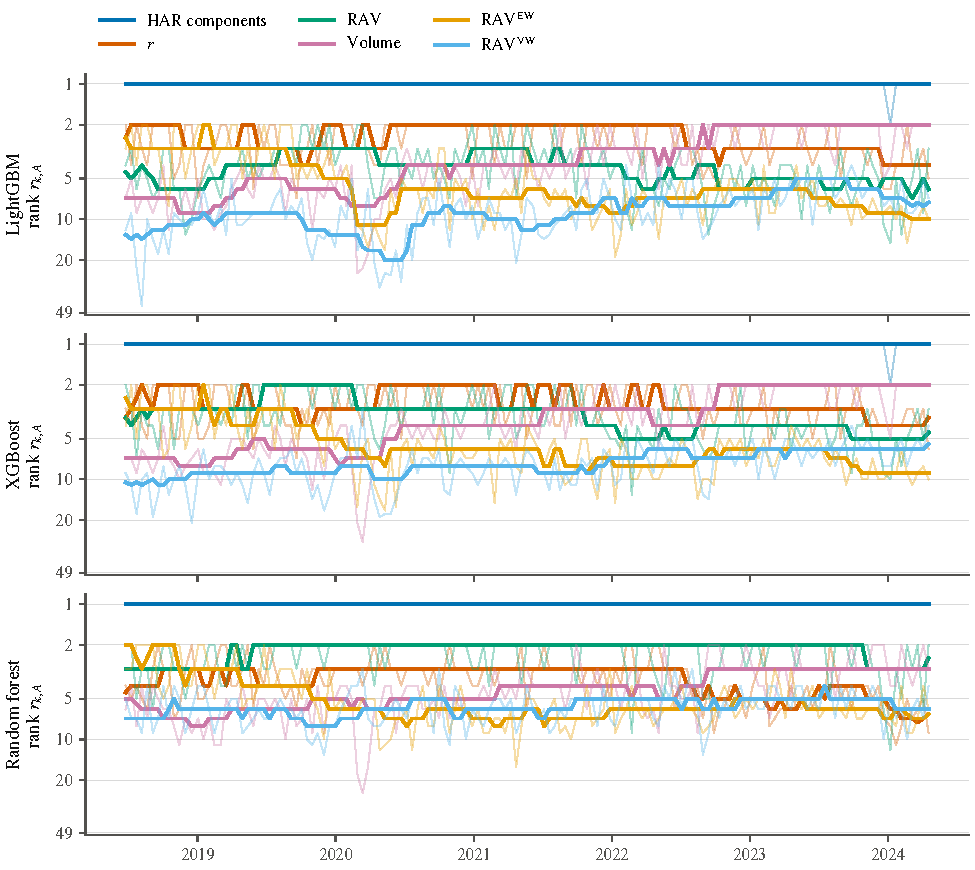
\includegraphics[width=\linewidth]{figures/rehaul_fi_tree_ranks.pdf}
\caption{The trees' per-refit SHAP ranks over time, the six units with the lowest mean rank averaged over the three models. Rank $r_{k,A}$ of unit $A$ among the 49 by mean $|\phi_{t,A}|$ on refit $k$'s held-out rows (1 = largest; log scale), at the start of each refit's tail. Thin: one point per refit; thick: centred rolling median over 11 refits (about 110 sessions). Kendall's $W$ over the 147 refits: LightGBM 0.57, XGBoost 0.60, random forest 0.62.}
\label{fig:rh_fi_ranks}
\end{figure}


% Trees: SHAP interactions (global, per refit) and the H-statistic cross-check
% AUTO-GENERATED by writeup/make_rehaul_fi.py -- do not edit; re-run the script.

\begin{table}[tbp]
\centering
\small
\setlength{\tabcolsep}{4pt}
\begin{threeparttable}
\caption{Trees: the strongest SHAP interactions, global and per refit, with the $H$-statistic cross-check.}
\label{tab:rh_fi_inter}
\begin{tabular}{@{}lrrrrr@{}}
\toprule
Pair & $\bar I$ ($\times 10^{3}$) & $\bar r$ & Top 10 (\%) & $H^2$ (\%) & $H^2_{\min}$ \\
\midrule
\multicolumn{6}{@{}l}{\textit{LightGBM}: series pairs} \\
HAR ladder $\times$ \texttt{sumabsret} & 12.64 & 1.7 & 100 & 0.33 & 0.19 \\
HAR ladder $\times$ \texttt{sumret} & 10.95 & 2.4 & 99 & 0.29 & 0.09 \\
HAR ladder $\times$ \texttt{sumvolume} & 6.62 & 6.3 & 88 & 0.05 & 0.05 \\
HAR ladder $\times$ \texttt{sumabsret\_ewstock} & 5.46 & 6.3 & 88 & 0.05 & 0.12 \\
HAR ladder $\times$ \texttt{stocktwits\_sentiment} & 4.70 & 14.4 & 67 & 0.06 & 0.17 \\
\multicolumn{6}{@{}l}{\textit{LightGBM}: column pairs} \\
\texttt{har\_ma\_1} $\times$ \texttt{har\_ma\_5} & 10.25 & -- & -- & 0.36 & 0.02 \\
\texttt{har\_ma\_1} $\times$ \texttt{har\_ma\_25} & 4.63 & -- & -- & 0.10 & 0.02 \\
\texttt{har\_ma\_5} $\times$ \texttt{adj\_sumabsret\_ma\_1} & 4.53 & -- & -- & 0.67 & 0.42 \\
\quad Probe floor & 0.49 & \multicolumn{2}{c}{$W = 0.45$} & & \\
\addlinespace[3pt]
\multicolumn{6}{@{}l}{\textit{XGBoost}: series pairs} \\
HAR ladder $\times$ \texttt{sumabsret} & 15.23 & 1.6 & 100 & 0.37 & 0.39 \\
HAR ladder $\times$ \texttt{sumret} & 11.03 & 2.5 & 100 & 0.68 & 0.21 \\
HAR ladder $\times$ \texttt{sumvolume} & 7.40 & 6.0 & 90 & 0.08 & 0.08 \\
HAR ladder $\times$ \texttt{sumabsret\_ewstock} & 5.92 & 5.3 & 93 & 0.06 & 0.17 \\
HAR ladder $\times$ \texttt{stocktwits\_sentiment} & 4.87 & 11.8 & 69 & 0.09 & 0.25 \\
\multicolumn{6}{@{}l}{\textit{XGBoost}: column pairs} \\
\texttt{har\_ma\_1} $\times$ \texttt{har\_ma\_5} & 9.95 & -- & -- & 0.39 & 0.02 \\
\texttt{har\_ma\_1} $\times$ \texttt{har\_ma\_25} & 4.99 & -- & -- & 0.14 & 0.02 \\
\texttt{har\_ma\_1} $\times$ \texttt{adj\_sumabsret\_ma\_5} & 4.94 & -- & -- & 0.28 & 0.43 \\
\quad Probe floor & 0.41 & \multicolumn{2}{c}{$W = 0.47$} & & \\
\addlinespace[3pt]
\multicolumn{6}{@{}l}{\textit{Random forest}: series pairs} \\
HAR ladder $\times$ \texttt{sumabsret} & 23.85 & 1.1 & 100 & 0.85 & 1.50 \\
HAR ladder $\times$ \texttt{sumret} & 9.13 & 3.5 & 99 & 0.20 & 0.48 \\
HAR ladder $\times$ \texttt{sumvolume} & 8.52 & 3.6 & 99 & 0.05 & 0.17 \\
HAR ladder $\times$ \texttt{sumabsret\_ewstock} & 6.87 & 4.6 & 99 & 0.06 & 0.33 \\
HAR ladder $\times$ \texttt{sumabsret\_vwstock} & 6.59 & 4.7 & 98 & 0.05 & 0.26 \\
\multicolumn{6}{@{}l}{\textit{Random forest}: column pairs} \\
\texttt{har\_ma\_1} $\times$ \texttt{har\_ma\_5} & 25.31 & -- & -- & 1.16 & 0.06 \\
\texttt{har\_ma\_1} $\times$ \texttt{adj\_sumabsret\_ma\_1} & 8.67 & -- & -- & 0.89 & 1.48 \\
\texttt{har\_ma\_1} $\times$ \texttt{adj\_sumabsret\_ma\_5} & 6.74 & -- & -- & 0.32 & 1.04 \\
\quad Probe floor & 0.50 & \multicolumn{2}{c}{$W = 0.57$} & & \\
\bottomrule
\end{tabular}
\begin{tablenotes}[flushleft]
\footnotesize
\item \textit{Notes:} SHAP interaction values $\phi_{t,jl}$ (path-dependent TreeSHAP, Lundberg et al.\ 2020; $\sum_l \phi_{t,jl} = \phi_{t,j}$) of the local refits on each refit's held-out rows, all 1{,}469 scored sessions. Series pair $(A, B)$: $\Phi_{t,AB} = \sum_{j\in A}\sum_{l\in B}(\phi_{t,jl} + \phi_{t,lj})$; $\bar I_{AB}$ = mean of $|\Phi_{t,AB}|$ over the scored sessions, $\times 10^{3}$, in the fit space of $\hat y$. Column pairs: $|\phi_{t,jl} + \phi_{t,lj}|$. $\bar r$ and top 10: the pair's mean rank and share of refits in the top 10 when the 1176 series pairs are ranked per refit by their mean $|\Phi_{t,AB}|$ on the refit's rows. $H^2$ (Friedman--Popescu): the variance of $\mathrm{PD}_{AB} - \mathrm{PD}_A - \mathrm{PD}_B$ as a share of the variance of $\mathrm{PD}_{AB}$, \%; $H^2_{\min}$: the same numerator over $\min(\mathrm{var}\,\mathrm{PD}_A, \mathrm{var}\,\mathrm{PD}_B)$, a ratio. Both pooled over 15 refits (every 10th), each on the 100 held-out sessions from its anchor as evaluation and background points; computed for each model's top 10 series and top 5 column pairs. Probe floor: median over the 49 probe fits of the largest $\bar I$ between the continuous noise column and a unit. $W$: Kendall's $W$ of the per-refit rankings of each model's top 50 pairs. XGBoost and the forest are refitted locally with other library versions than the stored refits (forecast gaps up to 0.17).
\end{tablenotes}
\end{threeparttable}
\end{table}


% Trees: series-level interaction heatmap
% 2026-10-15 (user): parked -- non-standard figure; focus on legible tables
% % AUTO-GENERATED by writeup/make_rehaul_fi.py -- do not edit; re-run the script.
\begin{figure}[tbp]
\centering
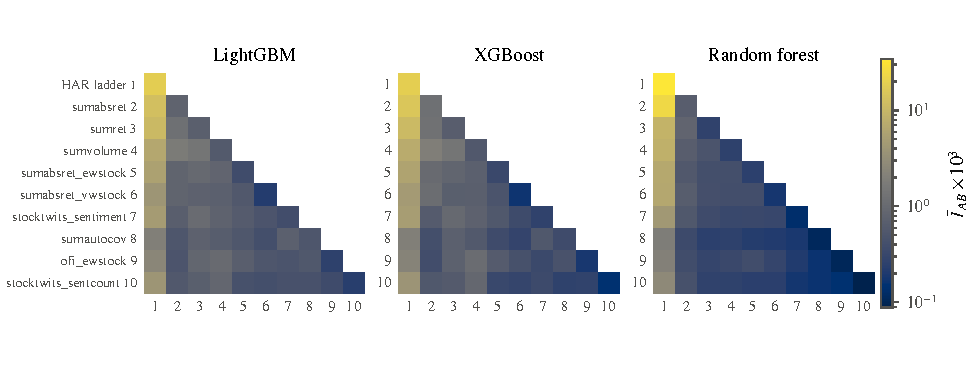
\includegraphics[width=\linewidth]{figures/rehaul_fi_inter_heatmap.pdf}
\caption{The trees' series-level SHAP interactions: $\bar I_{AB}$, the mean over the 1{,}469 scored sessions of $|\phi_{t,AB}|$, $\phi_{t,AB} = \sum_{j\in A}\sum_{l\in B}(\phi_{t,jl} + \phi_{t,lj})$, $\times 10^{3}$, log colour scale shared by the panels; lower triangle, the diagonal is the interaction among a unit's own columns, $\sum_{j \ne l \in A}\phi_{t,jl}$. Units: the 10 with the largest share of their model's off-diagonal interaction mass, summed over the three models; numbered as in the left panel. Local refits on the held-out rows of each of the 147 refits.}
\label{fig:rh_fi_inter}
\end{figure}

